\DiaryEntry{ODEs - Predator-Prey}{2018-07-30}{ODE}

The predator-prey system is a system of 2 ODEs with $R(t)$ denoting the amount of prey and $F(t)$ denoting the amount of predators. A simple model governing the population change over time is

\begin{align*}
\frac{dR}{dt} &= 2R - 1.2RF \\
\frac{dF}{dt} &= -F + 0.9RF
\end{align*}

In the first equation, the $2F$ term models the exponential growth of prey, when there are no predators, whereas the -1.2RF term corresponds to the negative effect on the prey of predator-prey interaction. In the second equation, the $-F$ term corresponds to the assumption that the predators die when there is no prey, whereas the $0.9RF$ term corresponds to the positive effect on the predators of the predator-prey interaction. The actual coefficients depend on the involved species.

To determine equilibrium conditions, we rewrite the system as

\begin{align*}
\frac{dR}{dt} &= R (2 - 1.2F) \\
\frac{dF}{dt} &= F(-1 + 0.9R)
\end{align*}

and solve for values of $R^\star,F^\star$ where the derivatives become zero,

\bee
2-1.2F^\star= 0 \rightarrow F^\star = 2/1.2, -1+0.9R^\star = 0 \rightarrow R^\star  = 1/0.9
\eee

Of course, another equilibrium solution is $R^\star= F^\star = 0$, i.e. no population at all.

The following Figure shows a plot of $R(t), F(t)$ for $R(t=0) = 1.0, F(t=0) = 0.5$.

\begin{figure}[H]
	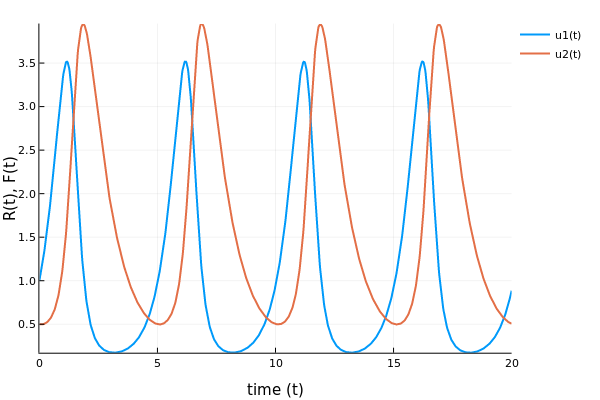
\includegraphics[scale=0.65]{images/ode_04_01.png}
\end{figure}

The solution is periodic and the peaks and lows of predator / prey are shifted: First the prey population increases which causes an increase in predators as well. When a certain number of predators is reached, the prey distribution decreases, causing a delayed decrease in predator population. With the chosen coefficients and initial conditions, the prey population comes very close to zero, but seems to recover and the cycle starts anew.

